\documentclass[11pt]{article}
\usepackage[T1]{fontenc}
\usepackage{lmodern}
\usepackage[margin=1in]{geometry}
\usepackage{amsmath,amssymb,amsthm,mathtools}
\usepackage{booktabs,array}
\usepackage{microtype}
\usepackage{tikz}
\usetikzlibrary{arrows.meta,calc,patterns,positioning}
\usepackage{float,needspace}
\usepackage[hidelinks]{hyperref}
\hypersetup{pdftitle={Exponential decay in two-dimensional classical O(n) models},
 pdfauthor={OpenAI}}
\newtheorem{theorem}{Theorem}[section]
\newtheorem{lemma}[theorem]{Lemma}
\newtheorem{proposition}[theorem]{Proposition}
\newtheorem{corollary}[theorem]{Corollary}
\theoremstyle{definition}
\newtheorem{definition}[theorem]{Definition}
\theoremstyle{remark}
\newtheorem{remark}[theorem]{Remark}
\newcommand{\E}{\mathbb E}
\newcommand{\R}{\mathbb R}
\newcommand{\Z}{\mathbb Z}
\newcommand{\N}{\mathbb N}
\newcommand{\C}{\mathbb C}
\newcommand{\HS}{\mathrm{HS}}
\newcommand{\dd}{\mathrm d}
\newcommand{\so}{\mathfrak{so}}
\numberwithin{equation}{section}
\clubpenalty=10000
\widowpenalty=10000
\setlength{\emergencystretch}{2em}

\title{Exponential decay in two-dimensional classical $O(n)$ models}
\author{OpenAI}
\date{September 23, 2026}

\begin{document}
\maketitle
\begin{abstract}
We prove exponential decay of two-point correlations for the classical
nearest-neighbor $O(n)$ model on the square lattice, for every $n\ge3$
and every finite positive inverse temperature. The estimate is uniform over
finite free-boundary subgraphs and bounded nonnegative edge strengths. This
resolves positively the all-temperature exponential spin-decay conjecture
for these models.
\end{abstract}

\section{Introduction}
\label{sec:introduction}

For the two-dimensional nearest-neighbor model, continuous symmetry
prevents spontaneous magnetization,
but it does not determine the rate at which distant spins decorrelate.
The central question for the classical $O(n)$ model is whether that
rate is exponential at every positive temperature when $n\ge3$.
We establish a finite-volume estimate that is uniform under deleting
vertices and edges and under weakening ferromagnetic couplings.

Let $G=(V,E)$ be a finite subgraph of the nearest-neighbor square lattice,
and let $b=(b_e)_{e\in E}$ satisfy $0\le b_e\le\beta<\infty$.
At each vertex put a spin $\sigma_x\in S^{n-1}$. Write
\begin{equation}
 \dd\mu_{G,b}^{(n)}(\sigma)
 =\frac{1}{Z_{G,b}^{(n)}}
   \exp\!\left(\sum_{\{x,y\}\in E}b_{xy}\sigma_x\cdot\sigma_y\right)
   \prod_{x\in V}\dd\omega_{n-1}(\sigma_x),
 \label{eq:model}
\end{equation}
where $\omega_{n-1}$ is uniform probability measure on the unit sphere.
There are no fixed boundary spins in \eqref{eq:model}, and no external
field or additional interaction. Expectations are denoted by
$\langle\,\cdot\,\rangle_{G,b}^{(n)}$.

\begin{theorem}
\label{thm:main}
For every integer $n\ge3$ and every finite $\beta>0$, there are constants
$A=A(n,\beta)<\infty$ and $m=m(n,\beta)>0$ such that, for every finite
nearest-neighbor square-lattice subgraph $G$, every strength array
$b\in[0,\beta]^E$, and all $x,y\in V$,
\begin{equation}
 0\le \langle\sigma_x\cdot\sigma_y\rangle_{G,b}^{(n)}
 \le A\exp(-m\|x-y\|_2).
 \label{eq:main-bound}
\end{equation}
\end{theorem}

\begin{corollary}[Free-boundary limits]\label{cor:limits}
Let $\Lambda_L=[-L,L]^2\cap\Z^2$, with all its nearest-neighbor edges,
free boundary conditions, and constant strength $\beta>0$. For every
$n\ge3$ and $x\in\Z^2$,
\begin{equation}
 \limsup_{L\to\infty}
 \left|\langle\sigma_0\cdot\sigma_x\rangle_{\Lambda_L,\beta}^{(n)}\right|
 \le A e^{-m\|x\|_2},
 \label{eq:limsup}
\end{equation}
with the constants of Theorem~\ref{thm:main}. Every subsequential local
weak limit of these laws satisfies the same two-point bound.
\end{corollary}

The volume-uniform estimate also gives finite spin susceptibility in
each limit from Corollary~\ref{cor:limits}: the sum
$\sum_{x\in\Z^2}\langle\sigma_0\cdot\sigma_x\rangle$
is bounded by $A\sum_{x\in\Z^2}e^{-m\|x\|_2}<\infty$.
The result concerns the spin two-point function. A full transfer gap
would additionally control covariances of all local observables,
including rotation-invariant bond energies, and requires a separate
argument. We do not identify the low-temperature correlation-length
asymptotic or prove uniqueness of infinite-volume Gibbs states.
The constants may deteriorate as $\beta\to\infty$.

\subsection{Historical context and the problem}

Mermin and Wagner proved the foundational no-order theorem for quantum
Heisenberg systems~\cite{MW}; Mermin then gave a direct classical
argument~\cite{Mermin1967}. McBryan and Spencer used complex spin
rotations to obtain algebraic upper bounds on two-dimensional
correlations~\cite{McBryanSpencer}. Gagnebin and Velenik extended this
approach to continuous interactions with much weaker regularity and
suitable long-range couplings~\cite{GagnebinVelenik}. Such bounds
quantify the loss of order but allow a zero exponential decay rate.

For two-component spins, this distinction is essential. The
Berezinskii--Kosterlitz--Thouless picture~\cite{Berezinskii,KosterlitzThouless}
includes a low-temperature phase with slow decay. Fr\"ohlich and
Spencer proved a polynomial lower bound for the ordinary plane rotator
at sufficiently low temperature~\cite[Theorem~C]{FS}. Their theorem
rules out an exponential upper bound in that regime, so
Theorem~\ref{thm:main} cannot extend to $n=2$.

For three or more components, Polyakov's non-Abelian renormalization
argument predicts mass generation at every positive
temperature~\cite{Polyakov}. Rigorous results have covered important
parts of this picture. Aizenman and Simon derived exponential decay
at high temperature from local Ward identities~\cite[Section~3]{AizenmanSimonWard}.
Kupiainen established an asymptotic $1/n$ expansion and proved a mass
gap in the corresponding large-component regime~\cite{Kupiainen}.
These regimes leave the question at a prescribed small spin dimension
and arbitrarily low positive temperature. Aru, Garban, and
Sep\'ulveda record the all-temperature lattice assertion as an open
conjecture in their 2025 study~\cite[Introduction, pp.~2--3]{AGS}.
Theorem~\ref{thm:main} resolves its spin-correlation formulation
positively for the free-boundary laws~\eqref{eq:model} and their
limits in Corollary~\ref{cor:limits}.

Geometric approaches illuminate a difficulty with reducing the number
of spin components. Conditioning one coordinate of a three-component
spin field gives a plane-rotator model with dependent random
couplings. Patrascioiu and Seiler investigated percolation of spin
regions as a route to a possible massless phase, with numerical and
conditional arguments for a constrained version of the
model~\cite{PatrascioiuSeiler}. Aru, Garban, and Sep\'ulveda constructed
random environments with predominantly strong couplings for which the
plane-rotator two-point function nevertheless decays exponentially
after averaging over the environment~\cite[Theorem~1.5]{AGS}.
Percolation of the strongly coupled region therefore does not by itself
force slow decay of these averaged correlations. In our argument the
three-component estimate is uniform over every strength array in
$[0,\beta]^E$; this uniformity permits the final conditional reduction
without assumptions on the distribution of the projected couplings.

\subsection{Methods and their ancestry}

Local rotation identities convert continuous symmetry into relations
among partition-function derivatives and correlations. Driessler, Landau, and
Perez used local Ward identities in estimates of critical lengths and
temperatures~\cite{DriesslerLandauPerez}. Aizenman and Simon also
obtained a finite-size criterion that turns sufficiently fast algebraic
decay into exponential decay for two, three, and four components
\cite[Section~4]{AizenmanSimonWard}. Such criteria separate the
large-distance argument from the task of proving adequate decay at
one finite scale. Here that task is carried out by a fourth variation
in two noncommuting rotation directions. The resulting family
inequality, combined with a range of spatial frequencies, controls a
boundary twist on an annulus. The required small quantity is the
probability that a sign cluster crosses that annulus.

The sign-cluster representation builds on several earlier constructions.
Ginibre's inequalities apply to the Ising and plane-rotator systems
that arise after conditioning spin amplitudes~\cite{Ginibre}.
The Fortuin--Kasteleyn representation and Edwards--Sokal coupling
relate ferromagnetic correlations to bond
connectivity~\cite{FortuinKasteleyn,EdwardsSokal}; Wolff's reflection
construction embeds such an Ising sign system in a continuous-spin
model~\cite{Wolff}. For three components, Campbell and Chayes proved
amplitude association, bond association, and boundary comparison,
and expressed a spin correlation as amplitude-weighted
connectivity~\cite[Lemma~2 and Corollaries~1, 3, and~4]{CC}.
We prove the finite-graph forms needed here and implement the boundary
comparison by pinning an arbitrary set of vertices simultaneously.
The reduction from $n$ components to three uses the same spherical
disintegration as the one-coordinate projection of
Aru--Garban--Sep\'ulveda~\cite[Proposition~2.4]{AGS}.

\subsection{Proof strategy and organization}

We first work with three-component spins. On a finite graph, rotating
spins by a spatially varying angle gives exact differentiation
identities for the partition function. Two different rotation axes
produce a response along their commutator axis. In
Proposition~\ref{prop:fourth}, summing the fourth derivative over a
family of test functions produces a nonnegative square plus controlled
local terms. The error bounds account for interactions among the test
functions; a suitable family will make those errors smaller than the
collective rotation response.
The bounds permit arbitrary prescribed boundary spins.

Section~\ref{sec:annulus} tests this inequality on a square annulus
whose boundary layers are pinned to two directions separated by an
angle $t$. Signed frequency families produce a factor $\log N$ in
the commutator field when the annulus has inner radius $N$.
Its quadratic response therefore gains $(\log N)^2$, while the total
error is only $O(\log N)$. This yields a one-sided curvature bound
for the positive, periodic boundary partition function $Z(t)$.
Integrating from a maximum proves that
$Z(\pi)/Z(0)\ge1-O_\beta(1/\log N)$, uniformly over all retained
vertices, edges, and strengths.

Section~\ref{sec:clusters} converts this analytic estimate into
exponential decay. The signs of one spin component form a
ferromagnetic Ising system when its absolute values are fixed. Open
bonds join equal signs, and their connected components carry
independent signs. Pinning both annular layers to the same pole
increases crossing probabilities; in the pinned system the crossing
probability is exactly $1-Z(\pi)/Z(0)$. Pinning the boundaries of
several disjoint annuli simultaneously makes their interiors
independent. Thus the probability that all are crossed is bounded by
a product of small probabilities. At one sufficiently large finite
scale, a sum over coarse paths gives a positive exponential rate.

Finally, conditioning on all coordinates after the third leaves
independent spherical reference directions in three dimensions and
weakens each coupling by a factor in $[0,1]$. The already uniform
three-component estimate survives this conditioning. This proves
Theorem~\ref{thm:main} for every integer $n\ge3$ and then
Corollary~\ref{cor:limits}.

\section{A fourth-order rotation estimate}
\label{sec:rotation}

The analytic input is a finite-graph inequality. Rotations about two
different axes produce a second-order effective rotation about a third
axis. A fourth variation of the partition function detects this effect;
after summing a family of test functions, its potentially large terms
form a nonnegative square. We establish the inequality with arbitrary
fixed boundary spins, as needed for the annuli below.

\subsection{Gauge invariance and second variations}

Local changes of spin variables underlie the Ward identities used
in~\cite{DriesslerLandauPerez,AizenmanSimonWard}; we begin with the
second-variation identity on a finite graph with prescribed spins.

Let \(G=(V,E)\) be a finite graph, with one orientation \(e=(x,y)\)
chosen for each edge, and let \(0\le b_e\le\beta\). Fix a set
\(P\subseteq V\) of vertices and arbitrary spins \(s_x\in S^2\) for
\(x\in P\). At the remaining vertices, integrate against uniform
probability measure on \(S^2\), with normalized density proportional to
\(\exp(\sum_{e=(x,y)}b_e s_x^Ts_y)\). Write \(\langle\cdot\rangle\)
for this expectation.

Let \(a,b,c\in\mathfrak{so}(3)\) denote cross product with the first,
second, and third coordinate vectors, respectively. Thus
\([a,b]=c\), and their operator norms are one. For an edge field
\(A=(A_e)_{e\in E}\) of skew matrices, put
\begin{equation}
\label{eq:rotation-partition}
\begin{split}
H(A)&=\sum_{e=(x,y)}b_e s_x^T\bigl(\exp(A_e)-I\bigr)s_y,\\
W(A)&=\bigl\langle\exp H(A)\bigr\rangle.
\end{split}
\end{equation}
Thus \(W\) is the ratio of the twisted partition function to the
untwisted one. All derivatives below are evaluated at \(A=0\). Set
\(X=DH\) and \(H_k=D^kH\) for \(k=2,3,4\). Compactness of the
finite spin space permits differentiation under the integral. We extend
all multilinear derivatives complex linearly in their arguments; changes
of spin variables themselves will always use real rotations.

For a scalar function on vertices, define \(df(e)=f_y-f_x\).
All scalar norms use counting measure on the indicated vertices or
edges. For a matrix indexed by edges,
\(\|T\|_{\mathrm{HS}}^2=\sum_{e,l\in E}|T_{el}|^2\).
For later use, the local derivative coefficients are
\begin{equation}
\label{eq:rotation-local-coefficients}
J_e(g_1,\ldots,g_k)
=b_e s_x^T\left(\frac{1}{k!}\sum_{\pi\in\mathfrak S_k}
g_{\pi(1)}\cdots g_{\pi(k)}\right)s_y,
\qquad |J_e(g_1,\ldots,g_k)|\le\beta,
\end{equation}
where each \(g_r\) is one of \(a,b,c\). Indeed, every matrix product
in this average has operator norm at most one. Consequently
\begin{equation}
\label{eq:rotation-local-expansion}
H_k(v_1g_1,\ldots,v_kg_k)
=\sum_e J_e(g_1,\ldots,g_k)\prod_{r=1}^k v_r(e).
\end{equation}
The coefficients depend on the spins and the generators, but not on the
scalar test functions. The same formula with \(k=1\) describes \(X\).

Define the complex bilinear form
\begin{equation}
\label{eq:rotation-R-definition}
R(h,k)=-D^2W(hc,kc)
\end{equation}
on scalar edge forms. It is symmetric, but is not assumed to be positive
semidefinite.

\begin{lemma}[Gradient estimates]\label{lem:gradient}
If \(f:V\to\mathbb C\) vanishes on \(P\), then, for
\(g\in\{a,b,c\}\),
\begin{equation}
\label{eq:rotation-gradient-bound}
\bigl\langle |X((df)g)|^2\bigr\rangle
\le\beta\|df\|_2^2.
\end{equation}
For every complex edge form \(h\),
\begin{equation}
\label{eq:rotation-R-bound}
R(h,\bar h)
=-\bigl\langle H_2(hc,\bar h c)+|X(hc)|^2\bigr\rangle
\le\beta\|h\|_2^2.
\end{equation}
Moreover, adding \(df\) in either argument of \(R\) does not change
its value whenever \(f\) vanishes on \(P\).
\end{lemma}

\begin{proof}
For real \(f\), make the change of variables
\(s_x^{\mathrm{old}}=\exp(-tf_xg)s_x^{\mathrm{new}}\) at every
integrated vertex. The fixed spins are unchanged because \(f|_P=0\).
Commutation of rotations about the same axis gives
\(W(t(df)g)=1\). Its second derivative at zero is
\[
0=\bigl\langle H_2((df)g,(df)g)+X((df)g)^2\bigr\rangle.
\]
The coefficient bound in \eqref{eq:rotation-local-coefficients} proves
\eqref{eq:rotation-gradient-bound} for real \(f\). For
\(f=f_1+if_2\), with \(f_1,f_2\) real, the squared modulus of
\(X((df)g)\) is the sum of the squares for \(f_1\) and \(f_2\).
Adding their bounds proves the complex case with the same constant.

Differentiating \eqref{eq:rotation-partition} twice gives the equality
in \eqref{eq:rotation-R-bound}. The local term is bounded in absolute
value by \(\beta\|h\|_2^2\), and the other term is nonnegative
before its minus sign, proving the inequality. Finally, the same change
of variables gives
\(W((h+df)c)=W(hc)\) for real \(h,f\). Differentiation in independent
scalar multiples of \(h\) and \(df\), followed by complex linear
extension, gives \(R(h,df)=R(df,h)=0\). This proves the last assertion.
\end{proof}

\subsection{The family inequality}

For vertex functions \(f,g\), write
\begin{equation}
\label{eq:rotation-S-definition}
S(f,g)_e=\tfrac12(f_xg_y-g_xf_y),\qquad e=(x,y).
\end{equation}
This form is bilinear and antisymmetric in \(f,g\).

\begin{proposition}[Fourth-order rotation inequality]\label{prop:fourth}
Let \((f_i)_{i\in I}\) be a finite family of complex vertex functions
vanishing on \(P\), and put
\[
u_i=df_i,\qquad
T_{el}=\sum_{i\in I}u_i(e)\overline{u_i(l)},\qquad
Q=\sum_{i\in I}S(f_i,\bar f_i).
\]
Then
\begin{equation}
\label{eq:rotation-family-bound}
\begin{split}
R(Q,\bar Q)
&\le K_{\mathrm{rot}}(\beta)\|T\|_{\mathrm{HS}}^2\\
&\quad+\beta\sum_{i,j\in I}
\min\bigl\{\|f_i\|_\infty^2\|df_j\|_2^2,
             \|f_j\|_\infty^2\|df_i\|_2^2\bigr\},
\end{split}
\end{equation}
where
\begin{equation}
\label{eq:rotation-explicit-constant}
K_{\mathrm{rot}}(\beta)=6\beta^2+4\beta^{3/2}+\beta.
\end{equation}
In particular, the constants are independent of the graph, the family
size, and the values of the fixed spins.
\end{proposition}

\begin{proof}
We first derive an exact identity relating the response \(R\) to a fourth
derivative of \(W\), and sum it over the family.  Gradient invariance will
control the resulting cross terms; a nonnegative square will supply the
remaining fourth-derivative lower bound.

\medskip\noindent
\emph{The noncommuting gauge identity.}
Let \(F_x\) be a real matrix potential in the span of \(a,b\), zero
on \(P\). The substitution
\(s_x^{\mathrm{old}}=\exp(-F_x)s_x^{\mathrm{new}}\) gives
\begin{equation}
\label{eq:rotation-nonabelian-gauge}
W(dF)=W(B),\qquad
B_e=\log\bigl(\exp(F_x)\exp(F_y-F_x)\exp(-F_y)\bigr)
\end{equation}
for \(F\) sufficiently small. The product inside the logarithm is
orthogonal and near the identity; hence its local logarithm is skew
symmetric. The logarithm also commutes with conjugation. Multiplying
the exponential series to degree two, and then taking the logarithm,
gives
\begin{equation}
\label{eq:rotation-B-quadratic}
B_e=\tfrac12[F_x,F_y]+O(F^3),\qquad DB_e(0)=0.
\end{equation}
For directions \(fa\) and \(gb\), the mixed second derivative of
\(B_e\) is therefore \(S(f,g)_e c\); it is zero for two directions
using the same generator.

We also need a fourth-order cancellation. Take four independent
parameters whose matrix directions have generator pattern \((a,b,a,b)\),
with arbitrary spatial potentials. The corresponding mixed fourth
derivative of \(B_e\) is zero. To see this, conjugate by the half-turn
about the first axis. This fixes \(a\) and negates \(b\), so the
coefficient involving all four parameters is fixed by conjugation:
its two \(b\)-directions contribute two minus signs. Conjugation by
the half-turn about the second axis likewise fixes this coefficient.
On \(\mathfrak{so}(3)\), the fixed spaces of these two conjugations
are respectively \(\mathbb R a\) and \(\mathbb R b\), with zero
intersection. Thus
\begin{equation}
\label{eq:rotation-B-fourth}
D_{1234}B_e=0
\quad\text{for the generator pattern }(a,b,a,b).
\end{equation}
Both \eqref{eq:rotation-B-quadratic} and
\eqref{eq:rotation-B-fourth} extend complex multilinearly. No complex
change of spin variables is involved in this extension.

For fixed \(i,j\), take the four edge directions
\begin{equation}
\label{eq:rotation-four-directions}
A_1=u_i a,\qquad A_2=\bar u_i b,\qquad
A_3=\bar u_j a,\qquad A_4=u_j b.
\end{equation}
The fourth derivative of the composition in
\eqref{eq:rotation-nonabelian-gauge} has no term containing \(DB\),
by \eqref{eq:rotation-B-quadratic}. Its term \(DW[D_{1234}B]\)
also vanishes, by \eqref{eq:rotation-B-fourth}. Only pairings of two
second derivatives remain. The pairing \(13|24\) is zero because
both pairs have the same generator. For the other two pairings, put
\(S_i=S(f_i,\bar f_i)\) and \(S_{ij}=S(f_i,f_j)\). Their arguments
are
\[
12|34:\quad(S_i c,\overline{S_j}c),\qquad
14|23:\quad(S_{ij}c,-\overline{S_{ij}}c).
\]
Here \(S(\bar f_j,f_j)=\overline{S_j}\) and
\(S(\bar f_j,\bar f_i)=-\overline{S_{ij}}\). Each labeled pairing
occurs once in the composition rule, so
\begin{equation}
\label{eq:rotation-fourth-identity}
D^4W(A_1,A_2,A_3,A_4)
=-R(S_i,\overline{S_j})+R(S_{ij},\overline{S_{ij}}).
\end{equation}
This also holds when some spatial functions coincide: the derivative
identity is multilinear in the four labeled directions.

Summing over \(i,j\) and rearranging gives the identity to be estimated:
\begin{equation}
\label{eq:rotation-response-balance}
R(Q,\bar Q)
=\sum_{i,j}R(S_{ij},\overline{S_{ij}})
 -\sum_{i,j}D^4W(u_i a,\bar u_i b,\bar u_j a,u_j b).
\end{equation}
We bound the first sum from above using gradient invariance, and the
second from below by retaining a nonnegative square.

\medskip\noindent
\emph{The cross terms.}
For functions \(f,g\) vanishing on \(P\), the product \(fg\)
also vanishes there, and the edge identities
\begin{equation}
\label{eq:rotation-gradient-adjustment}
\begin{split}
S(f,g)+\tfrac12d(fg)&=\tfrac12(f_x+f_y)\,dg,\\
S(f,g)-\tfrac12d(fg)&=-\tfrac12(g_x+g_y)\,df
\end{split}
\end{equation}
hold on \(e=(x,y)\). Applying gradient invariance in both arguments
of \(R\), followed by \eqref{eq:rotation-R-bound}, gives
\begin{equation}
\label{eq:rotation-cross-bound}
R(S(f,g),\overline{S(f,g)})
\le\beta\min\{\|f\|_\infty^2\|dg\|_2^2,
                 \|g\|_\infty^2\|df\|_2^2\}.
\end{equation}

\medskip\noindent
\emph{The fourth-derivative lower bound.}
We claim that
\begin{equation}
\label{eq:rotation-fourth-lower}
\sum_{i,j}D^4W(u_i a,\bar u_i b,\bar u_j a,u_j b)
\ge-K_{\mathrm{rot}}(\beta)\|T\|_{\mathrm{HS}}^2.
\end{equation}
To enumerate its terms, set \(X_r=X(A_r)\), and write
\(H_{r_1\cdots r_k}=H_k(A_{r_1},\ldots,A_{r_k})\). Direct
differentiation of \(\exp H\) gives all fifteen set partitions:
\begin{equation}
\label{eq:rotation-fifteen-terms}
\begin{aligned}
D^4W(A_1,A_2,A_3,A_4)=\bigl\langle
&X_1X_2X_3X_4\\
&+H_{12}X_3X_4+H_{13}X_2X_4+H_{14}X_2X_3\\
&+H_{23}X_1X_4+H_{24}X_1X_3+H_{34}X_1X_2\\
&+H_{12}H_{34}+H_{13}H_{24}+H_{14}H_{23}\\
&+H_{123}X_4+H_{124}X_3+H_{134}X_2+H_{234}X_1\\
&+H_{1234}\bigr\rangle.
\end{aligned}
\end{equation}
The four terms comprising
\((X_1X_2+H_{12})(X_3X_4+H_{34})\), after summation over \(i,j\),
have expectation
\begin{equation}
\label{eq:rotation-positive-square}
\left\langle\left|\sum_i
\bigl[X(u_i a)X(\bar u_i b)+H_2(u_i a,\bar u_i b)\bigr]
\right|^2\right\rangle\ge0.
\end{equation}
We bound the other eleven terms in absolute value.

For an edge \(e\), let \(t_e(l)=T_{el}\) and
\(\rho_e=(\sum_l|T_{el}|^2)^{1/2}\), and abbreviate
\(X_g(v)=X(vg)\). Crucially,
\begin{equation}
\label{eq:rotation-row-gradient}
t_e=d\left(\sum_i u_i(e)\overline{f_i}\right).
\end{equation}
The potential on the right, and its conjugate, vanish on \(P\).
Lemma~\ref{lem:gradient} therefore gives
\begin{equation}
\label{eq:rotation-row-bound}
\langle|X_g(t_e)|^2\rangle\le\beta\rho_e^2,
\qquad
\langle|X_g(\bar t_e)|^2\rangle\le\beta\rho_e^2.
\end{equation}

The following table records every remaining contraction. Expand each
\(H_k\) using \eqref{eq:rotation-local-expansion}, sum over \(i,j\),
and multiply the last two columns. One then sums over \(e\), except
in the two \(H_2H_2\) rows, where one sums over \(e,l\).
\begin{center}
\renewcommand{\arraystretch}{1.18}
\begin{tabular}{@{}lll@{}}
\toprule
Term & Local coefficient & Contracted expression\\
\midrule
\(H_{13}X_2X_4\) & \(J_e(a,a)\)
  & \(X_b(t_e)X_b(\bar t_e)\)\\
\(H_{14}X_2X_3\) & \(J_e(a,b)\)
  & \(X_b(t_e)X_a(t_e)\)\\
\(H_{23}X_1X_4\) & \(J_e(b,a)\)
  & \(X_a(\bar t_e)X_b(\bar t_e)\)\\
\(H_{24}X_1X_3\) & \(J_e(b,b)\)
  & \(X_a(\bar t_e)X_a(t_e)\)\\
\midrule
\(H_{13}H_{24}\) & \(J_e(a,a)J_l(b,b)\)
  & \(T_{el}\overline{T_{el}}\)\\
\(H_{14}H_{23}\) & \(J_e(a,b)J_l(b,a)\)
  & \(T_{el}^{\,2}\)\\
\midrule
\(H_{123}X_4\) & \(J_e(a,b,a)\)
  & \(T_{ee}X_b(\bar t_e)\)\\
\(H_{124}X_3\) & \(J_e(a,b,b)\)
  & \(T_{ee}X_a(t_e)\)\\
\(H_{134}X_2\) & \(J_e(a,a,b)\)
  & \(T_{ee}X_b(t_e)\)\\
\(H_{234}X_1\) & \(J_e(b,a,b)\)
  & \(T_{ee}X_a(\bar t_e)\)\\
\midrule
\(H_{1234}\) & \(J_e(a,b,a,b)\) & \(T_{ee}^{\,2}\)\\
\bottomrule
\end{tabular}
\end{center}
For example, the first row follows from
\[
\begin{split}
&\sum_{i,j}u_i(e)\bar u_j(e)
             X_b(\bar u_i)X_b(u_j)\\
&\qquad=
X_b\left(\sum_i u_i(e)\bar u_i\right)
X_b\left(\sum_j\bar u_j(e)u_j\right)
=X_b(t_e)X_b(\bar t_e).
\end{split}
\]
The other rows follow by the same finite summation; their explicit
expressions distinguish the conjugated and unconjugated contractions.

For each of the first four rows, the pointwise coefficient bound and
Cauchy--Schwarz, followed by \eqref{eq:rotation-row-bound}, give an
absolute expectation at edge \(e\) of at most
\(\beta^2\rho_e^2\). The coefficient may depend on the spins;
its pointwise absolute value is bounded before applying
Cauchy--Schwarz. These four rows contribute at most
\(4\beta^2\|T\|_{\mathrm{HS}}^2\).
The next two rows contribute at most
\(2\beta^2\|T\|_{\mathrm{HS}}^2\), since both contractions have
absolute value \(|T_{el}|^2\).

For each of the four \(H_3X\) rows,
\eqref{eq:rotation-row-bound} bounds the total absolute expectation by
\[
\beta^{3/2}\sum_e T_{ee}\rho_e
\le\beta^{3/2}
\left(\sum_e T_{ee}^2\right)^{1/2}
\left(\sum_e\rho_e^2\right)^{1/2}
\le\beta^{3/2}\|T\|_{\mathrm{HS}}^2.
\]
Here \(T_{ee}=\sum_i|u_i(e)|^2\ge0\), and the squared diagonal
entries form part of the Hilbert--Schmidt sum. The last row is bounded
by \(\beta\sum_e T_{ee}^2\le\beta\|T\|_{\mathrm{HS}}^2\).

Finally, the sum on the left of \eqref{eq:rotation-fourth-lower} is
real: complex conjugation interchanges \(i,j\) and permutes the
arguments of the symmetric fourth derivative. Keeping the nonnegative
square \eqref{eq:rotation-positive-square}, and subtracting the bounds
for the remaining terms, proves \eqref{eq:rotation-fourth-lower} with
exactly \(K_{\mathrm{rot}}(\beta)\) from
\eqref{eq:rotation-explicit-constant}.

Combining \eqref{eq:rotation-cross-bound} and
\eqref{eq:rotation-fourth-lower} in
\eqref{eq:rotation-response-balance} proves
\eqref{eq:rotation-family-bound}. Only the upper bound and gradient
invariance of \(R\) were used; no positivity property of \(R\) is
required.
\end{proof}

\section{A uniform estimate for an annular twist}\label{sec:annulus}

We apply the fourth-variation estimate to an annulus with two prescribed
boundary directions.  The aim is to bound uniformly how much its partition
function changes when one boundary direction rotates.  The spatial tests
will be defined on the full annulus and then restricted to the retained
graph.
In this section, $C$ denotes a finite constant depending only on the
fixed smooth profiles, and $C_\beta$ may also depend on $\beta$;
these constants may increase from one estimate to the next.

For an integer $N\geq 2$, let
\[
 D_N=\{x\in\Z^2:N\leq\|x\|_\infty\leq 2N\}.
\]
Let $G=(V,E)$ be any subgraph of the nearest-neighbor graph on $D_N$,
and orient each edge in a positive coordinate direction.  Give its edges
strengths $0\leq b_e\leq\beta$.  Put $s_*=(1,0,0)$ and prescribe
\[
 s_x=\exp(tc)s_*\quad(\|x\|_\infty=N),
 \qquad
 s_x=s_*\quad(\|x\|_\infty=2N)
 \quad (x\in V).
\]
All other spins are integrated against uniform probability measure on
$S^2$.  Write $Z(t)$ for the resulting partition integral, including the
interactions between any prescribed spins.  Missing vertices on either
boundary require no additional convention: only vertices of $V$ are
pinned.

\begin{proposition}[Vanishing annular twist cost]\label{prop:annulus}
For every finite $\beta>0$ there is a finite constant $C_\beta$ such that,
for all $N\geq2$ and all graphs and strengths just described,
\begin{equation}\label{eq:annulus-minmax}
 \frac{\min_{t\in\R}Z(t)}{\max_{t\in\R}Z(t)}
 \geq 1-\frac{C_\beta}{\log N}.
\end{equation}
In particular,
\begin{equation}\label{eq:annulus-ratio}
 \frac{Z(\pi)}{Z(0)}\geq1-\frac{C_\beta}{\log N}.
\end{equation}
The constant is independent of the subgraph, the strength array, and
the twist parameter.
\end{proposition}

\subsection{Boundary gauge and multiscale tests}

Fix once and for all a real smooth function $\Theta$ equal to one in a
neighborhood of $[-1,1]^2$ and compactly supported in $(-2,2)^2$.  Define
the real edge form
\begin{equation}\label{eq:annulus-h}
 h_e=\Theta(y/N)-\Theta(x/N),\qquad e=(x,y).
\end{equation}
Use a subscript $t$ on $W,X,H_k,R$ for the quantities from the preceding
section evaluated with these boundary values, and write
$\langle\,\cdot\,\rangle_t$ for the corresponding expectation.  Although
$\Theta$ does not vanish on the inner pinned layer, its gauge action is
still explicit:
\begin{equation}\label{eq:annulus-boundary-gauge}
 W_t(shc)=\frac{Z(t+s)}{Z(t)},
 \qquad
 R_t(h,h)=-\frac{Z''(t)}{Z(t)}.
\end{equation}
Indeed, substituting
$s_x^{\mathrm{old}}=\exp(-s\Theta(x/N)c)s_x^{\mathrm{new}}$
cancels every edge matrix.  It changes the inner boundary value to
$\exp((t+s)c)s_*$ and leaves the outer value unchanged.  Thus the gauge
changes the prescribed boundary values, rather than treating them as
integrated variables.

The analytic target is now an upper bound of order $1/\log N$ for
$R_t(h,h)$.  We will construct functions whose collective form
$\sum_i S(f_i,\overline{f_i})$ equals $-i\lambda_N\widetilde h$,
where $\lambda_N\geq\tfrac12\log N$ and $\widetilde h$ approximates $h$.
The two family costs in Proposition~\ref{prop:fourth} will total
$O(\log N)$, whereas bilinearity multiplies
$R_t(\widetilde h,\widetilde h)$ by $\lambda_N^2$.
This yields the required logarithmic gain; after constructing the family,
we will transfer the bound from $\widetilde h$ to $h$ without assuming
that $R_t$ is positive.

For $m=1,2$, put $g_m=\partial_m\Theta$.  Choose a real smooth cutoff
$\chi_m$ compactly supported in
\[
 \mathcal A=\{z\in\R^2:1<\|z\|_\infty<2\}
\]
and equal to one on $\operatorname{supp}g_m$.  Such a cutoff exists
because $g_m$ vanishes near both boundary squares.  The real profiles
\begin{equation}\label{eq:annulus-profiles}
 \phi_{m,+}=\frac{\chi_m+g_m}{2},\qquad
 \phi_{m,-}=\frac{\chi_m-g_m}{2}
 \quad\hbox{satisfy}\quad
 \phi_{m,+}^2-\phi_{m,-}^2=g_m.
\end{equation}
This construction uses no square root of a signed smooth function.
All four profiles have compact support in $\mathcal A$.
Figure~\ref{fig:annulus-tests} shows how these supports lie between
the two pinned layers.

\begin{figure}[htbp]
\centering
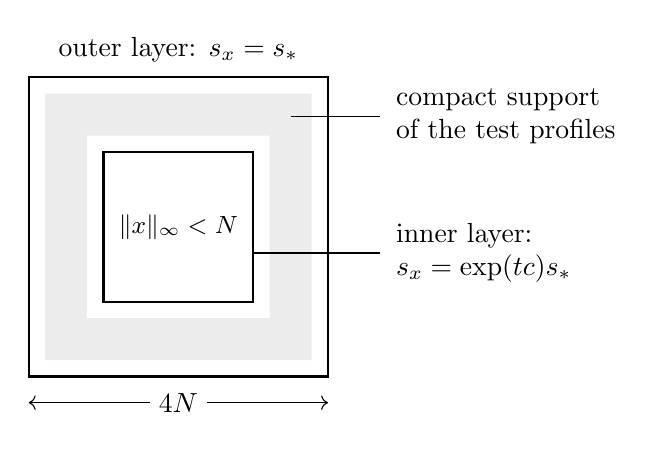
\begin{tikzpicture}[scale=0.95]
 \path[fill=gray!15,even odd rule]
   (-1.78,-1.78) rectangle (1.78,1.78)
   (-1.22,-1.22) rectangle (1.22,1.22);
 \draw[thick] (-2,-2) rectangle (2,2);
 \draw[thick] (-1,-1) rectangle (1,1);
 \node[font=\small] at (0,0) {$\|x\|_\infty<N$};
 \node[anchor=south] at (0,2.08)
   {outer layer: $s_x=s_*$};
 \draw (1,-0.35) -- (2.7,-0.35);
 \node[anchor=west,align=left] at (2.78,-0.35)
   {inner layer:\\$s_x=\exp(tc)s_*$};
 \draw (1.5,1.48) -- (2.7,1.48);
 \node[anchor=west,align=left] at (2.78,1.48)
   {compact support\\of the test profiles};
 \draw[<->] (-2,-2.35) -- (2,-2.35);
 \node[fill=white] at (0,-2.35) {$4N$};
\end{tikzpicture}
\caption{The boundary twist is tested using profiles supported strictly
between the pinned squares.  The shaded region is schematic: one fixed
compact subannulus contains all four profile supports.  The estimates
remain valid when arbitrary vertices and edges are deleted.}
\label{fig:annulus-tests}
\end{figure}

For $p\in\Z^2$ let $r_p=\|p\|_\infty$.  Introduce four groups of
vertex functions, restricted to $V$:
\begin{equation}\label{eq:annulus-modes}
 f_{m,\pm,p}(x)
 =r_p^{-3/2}\phi_{m,\pm}(x/N)
       \exp\left(\frac{2\pi i\,p\cdot x}{16N}\right),
 \qquad
 1\leq r_p\leq N,\quad \pm p_m>0.
\end{equation}
They vanish at every pinned vertex.  The power $r_p^{-3/2}$ is chosen
to produce a harmonic sum: the shell face $p_m=\pm r$ contains $2r+1$ modes, each with
squared normalization $r^{-3}$ and coordinate-$m$ phase increment of order
$r/N$.  Its summed frequency factor in the commutator is therefore of
order $1/(Nr)$.  The opposite frequency signs give the adjacent-point
products of $\phi_{m,+}$ and $\phi_{m,-}$ opposite coefficients.
Index this finite family by $i$, write $u_i=df_i$, and, as in
Proposition~\ref{prop:fourth}, put
\[
 T_{e\ell}=\sum_i u_i(e)\overline{u_i(\ell)},
 \qquad
 S(f,g)_e=\tfrac12(f_xg_y-g_xf_y).
\]
For an edge $e=(x,x+e_m)$ define
\begin{equation}\label{eq:annulus-htilde}
 \widetilde h_e=\frac1N
 \left[
 \phi_{m,+}(x/N)\phi_{m,+}((x+e_m)/N)
 -\phi_{m,-}(x/N)\phi_{m,-}((x+e_m)/N)
 \right].
\end{equation}

\begin{lemma}[The multiscale family]\label{lem:modes}
There is a constant $C$, depending only on the fixed profiles, with the
following properties for every $N\geq2$ and every such subgraph.
First,
\begin{equation}\label{eq:annulus-commutator}
 \sum_i S(f_i,\overline{f_i})=-i\lambda_N\widetilde h,
 \qquad
 \lambda_N
 =N\!\!\sum_{\substack{1\leq r_p\leq N\\p_1>0}}
      r_p^{-3}\sin\left(\frac{2\pi p_1}{16N}\right)
 \geq\frac12\sum_{r=1}^N\frac1r.
\end{equation}
Second,
\begin{equation}\label{eq:annulus-midpoint}
 \|h\|_2\leq C,\qquad
 \|h+\widetilde h\|_\infty\leq\frac CN,\qquad
 \|h-\widetilde h\|_1\leq\frac CN.
\end{equation}
Finally,
\begin{equation}\label{eq:annulus-test-cost}
 \|T\|_{\mathrm{HS}}^2+
 \sum_{i,j}\min\left\{
   \|f_i\|_\infty^2\|df_j\|_2^2,
   \|f_j\|_\infty^2\|df_i\|_2^2
 \right\}
 \leq C(1+\log N).
\end{equation}
All edge norms use counting measure on $E$.
\end{lemma}

\begin{proof}
For a real profile $\phi$ and one mode on shell $r_p$, direct substitution
on a positive coordinate-$j$ edge gives
\begin{equation}\label{eq:annulus-one-mode}
 S(f_p,\overline{f_p})_e
 =-i r_p^{-3}\phi(x/N)\phi((x+e_j)/N)
       \sin\left(\frac{2\pi p_j}{16N}\right).
\end{equation}
If the group is indexed by $m\ne j$, its frequency set is invariant
under $p_j\mapsto-p_j$, so its sum vanishes.  For $m=j$, the negative
half-plane gives the negative of the positive-half-plane sine sum.
Interchanging coordinates identifies the positive sums for $j=1,2$.
This proves the identity in \eqref{eq:annulus-commutator}.

On shell $r$, retain only the $2r+1$ frequencies with $p_1=r$ and
$|p_2|\leq r$.  Since
\[
 \sin\left(\frac{\pi r}{8N}\right)\geq\frac r{4N}
 \qquad(1\leq r\leq N),
\]
their contribution to $\lambda_N$ is at least
$(2r+1)/(4r^2)\geq1/(2r)$.  This gives its asserted lower bound.

For an edge in direction $m$, let $z=(x+y)/(2N)$.  Centered Taylor
expansion, with uniform bounds on the fixed smooth functions, gives
\[
 h_e=N^{-1}\partial_m\Theta(z)+O(N^{-3}),\qquad
 \phi(x/N)\phi(y/N)=\phi(z)^2+O(N^{-2}).
\]
Using \eqref{eq:annulus-profiles} yields
$|h_e-\widetilde h_e|\leq C N^{-3}$.  There are $O(N^2)$ annulus
edges, and $|h_e|+|\widetilde h_e|\leq C/N$.  The three estimates in
\eqref{eq:annulus-midpoint} follow, also after restriction to $E$.

For a mode on shell $r$, the product rule for a discrete difference
and $|e^{iv}-1|\leq|v|$ give
\begin{equation}\label{eq:annulus-mode-norms}
 \|f_i\|_\infty\leq Cr^{-3/2},\qquad
 \|df_i\|_2\leq Cr^{-3/2}(1+r)\leq C' r^{-1/2}.
\end{equation}
There are $O(r)$ modes on shell $r$, including all four groups.
For shells $s\leq r$, choose the bound in the minimum that uses the
supremum norm of the shell-$r$ mode.  The cost of a pair is at most
$Cr^{-3}s^{-1}$; all $O(rs)$ pairs therefore cost at most $Cr^{-2}$.
Summing both shell orderings gives
\begin{equation}\label{eq:annulus-minimum-sum}
 \sum_{i,j}\min\left\{
   \|f_i\|_\infty^2\|df_j\|_2^2,
   \|f_j\|_\infty^2\|df_i\|_2^2
 \right\}
 \leq C\sum_{r=1}^N\sum_{s=1}^r r^{-2}
 \leq C'(1+\log N).
\end{equation}

It remains to bound $T$.  Applying the triangle inequality mode by mode
would give only $\|T\|_{\mathrm{HS}}\leq\sum_i\|df_i\|_2^2=O(N)$;
we use Fourier orthogonality for the sharper bound.  Work first in a
single profile group and let $U$ be the matrix whose $p$-th column is
$r_p^{1/2}df_p$.
Embed the annulus in the discrete torus
$Q_N=(\Z/(16N)\Z)^2$.  Its representatives may be chosen in
$[-8N,8N-1]^2$; all profiles vanish near the boundary of this square,
so they also define torus functions.  Let $F$ have columns
\[
 F_{x,p}=\exp\left(\frac{2\pi i\,p\cdot x}{16N}\right),
 \qquad x\in Q_N,
\]
using the frequencies of this group.  They are distinct modulo $16N$,
and orthogonality of these unnormalized waves gives
\begin{equation}\label{eq:annulus-fourier-norm}
 F^*F=(16N)^2I,\qquad \|F\|_{\mathrm{op}}=16N.
\end{equation}
For direction $j$, let $P_j$ restrict functions on $Q_N$ to the
origins of the coordinate-$j$ edges in $E$.  Let $M_v$ denote
multiplication by $v$ on $Q_N$, and set
\[
 \Delta_j\phi(x)=\phi((x+e_j)/N)-\phi(x/N),
 \qquad \phi^{(j)}(x)=\phi((x+e_j)/N).
\]
The directional block of $U$ has the exact factorization
\begin{align}\label{eq:annulus-operator-factorization}
 U_j={}&P_jM_{\Delta_j\phi}F
              \operatorname{diag}(r_p^{-1})\notag\\
 &+P_jM_{\phi^{(j)}}F
   \operatorname{diag}\left(
      \frac{\exp(2\pi i p_j/(16N))-1}{r_p}\right).
\end{align}
Here $\|P_j\|_{\mathrm{op}}\leq1$,
$\|\Delta_j\phi\|_\infty\leq C/N$, and the last diagonal factor
has operator norm at most $C/N$, since $|p_j|\leq r_p$.
Equation~\eqref{eq:annulus-fourier-norm} now gives
$\|U_j\|_{\mathrm{op}}\leq C$ and hence
$\|U\|_{\mathrm{op}}\leq C$ after combining the two directions.

The contribution of this group is
\[
 T_{\mathrm{group}}=U\operatorname{diag}(r_p^{-1})U^*.
\]
The finite-matrix inequality
$\|ADB\|_{\mathrm{HS}}\leq
\|A\|_{\mathrm{op}}\|D\|_{\mathrm{HS}}\|B\|_{\mathrm{op}}$
therefore implies
\[
 \|T_{\mathrm{group}}\|_{\mathrm{HS}}^2
 \leq C\sum_p r_p^{-2}
 \leq C'\sum_{r=1}^N r\,r^{-2}
 \leq C''(1+\log N).
\]
The triangle inequality over the four groups gives the same order
for $\|T\|_{\mathrm{HS}}^2$.  Together with
\eqref{eq:annulus-minimum-sum}, this proves
\eqref{eq:annulus-test-cost}.
\end{proof}

\subsection{From the test form to the boundary twist}

\begin{proof}[Proof of Proposition~\ref{prop:annulus}]
Apply Proposition~\ref{prop:fourth} in the law with twist $t$, using
the family \eqref{eq:annulus-modes}.  The left side is
\[
 R_t(-i\lambda_N\widetilde h,i\lambda_N\widetilde h)
 =\lambda_N^2R_t(\widetilde h,\widetilde h),
\]
because $R_t$ is bilinear and $\widetilde h$ is real.
Lemma~\ref{lem:modes} gives, uniformly in $t$,
\begin{equation}\label{eq:annulus-tested-response}
 R_t(\widetilde h,\widetilde h)
 \leq\frac{C_\beta(1+\log N)}{(\log N)^2}
 \leq\frac{C'_\beta}{\log N}.
\end{equation}

We must transfer this upper bound to $h$ without treating $R_t$ as a
positive form.  If $R_t(h,h)\leq0$, the desired positive upper bound
already holds.  Otherwise, the defining second-derivative identity
and the pointwise bound on $H_{2,t}$ give
\begin{equation}\label{eq:annulus-current-control}
 \langle X_t(hc)^2\rangle_t
 <-\langle H_{2,t}(hc,hc)\rangle_t
 \leq\beta\|h\|_2^2\leq C\beta.
\end{equation}
Put $d=h-\widetilde h$.  The current is a real random variable on
real edge forms, and
\[
 |X_t(dc)|\leq\beta\|d\|_1\leq\frac{C\beta}{N}.
\]
Consequently ordinary Cauchy--Schwarz for random variables, followed
by \eqref{eq:annulus-current-control}, yields
\begin{align}\label{eq:annulus-current-error}
 \left|\langle X_t(hc)^2-X_t(\widetilde h c)^2\rangle_t\right|
 &\leq
 2\langle X_t(hc)^2\rangle_t^{1/2}
       \|X_t(dc)\|_\infty+\|X_t(dc)\|_\infty^2\notag\\
 &\leq\frac{C_\beta}{N}.
\end{align}
The local quadratic term satisfies the stronger pointwise bound
\begin{align}\label{eq:annulus-local-error}
 |H_{2,t}(hc,hc)-H_{2,t}(\widetilde h c,\widetilde h c)|
 &\leq\beta\sum_{e\in E}|d_e|\,|h_e+\widetilde h_e|\notag\\
 &\leq\frac{C\beta}{N^2}.
\end{align}
Equations~\eqref{eq:annulus-tested-response}--\eqref{eq:annulus-local-error}
and the formula for $R_t$ imply in both cases that
\begin{equation}\label{eq:annulus-ode}
 -\frac{Z''(t)}{Z(t)}=R_t(h,h)
 \leq\frac{C_\beta}{\log N}+\frac{C_\beta}{N}
 \leq\delta_N,\qquad
 \delta_N=\frac{C'_\beta}{\log N}.
\end{equation}
All constants are independent of the boundary twist, the retained
vertices and edges, and the admissible strengths.

Finally, $Z$ is positive, smooth, and $2\pi$-periodic.  Set
$M=\max_t Z(t)$ and choose $t_0$ with $Z(t_0)=M$.  Then
$Z'(t_0)=0$, and \eqref{eq:annulus-ode} implies
$Z''(t)\geq-\delta_N Z(t)\geq-\delta_N M$.
For any $t$, choose an orientation $\epsilon\in\{-1,1\}$ and
$0\leq\ell\leq\pi$ with $t=t_0+\epsilon\ell$ modulo $2\pi$.
Twice integrating the second-derivative bound for
$v\mapsto Z(t_0+\epsilon v)$ gives
\[
 Z(t)\geq M-\frac{\delta_N M\ell^2}{2}
 \geq M\left(1-\frac{\pi^2\delta_N}{2}\right).
\]
Taking the minimum and enlarging $C_\beta$ proves
\eqref{eq:annulus-minmax}.  Since
$Z(\pi)/Z(0)\geq\min Z/\max Z$, it also proves
\eqref{eq:annulus-ratio}.
\end{proof}

\section{Sign clusters and exponential decay}\label{sec:clusters}

We now turn the uniform annulus estimate into a bound on connections.
The argument uses sign clusters, of the type studied for continuous-spin
systems in~\cite{CC}.  We prove the finite-volume comparison statements
needed here, including the comparison with pinned spins.

We return to the free spin law \eqref{eq:model} and its expectation
$\langle\cdot\rangle_{G,b}^{(n)}$, now on an arbitrary finite graph
$G=(V,E)$ with strengths $b_e\in[0,\beta]$.
Until the final subsection, $n=3$ and we write the spins as $s_x$.

\subsection{An associated amplitude and bond law}

Write
\begin{equation}\label{eq:spin-disintegration}
 s_x=(r_x\tau_x,q_x\cos\theta_x,q_x\sin\theta_x),
 \qquad q_x=(1-r_x^2)^{1/2}.
\end{equation}
Under the reference measure, the variables $r_x$, $\tau_x$, and
$\theta_x$ are independent and uniform on $[0,1]$, $\{-1,1\}$, and
$\R/(2\pi\Z)$, respectively.  Indeed, the first coordinate of a uniform
point on $S^2$ is uniform on $[-1,1]$, independently of its azimuthal
angle.  Conditional on all the amplitudes $r=(r_x)_{x\in V}$, the signs
and angles are independent Gibbs systems with respective couplings
\begin{equation}\label{eq:amplitude-couplings}
 K_{xy}=b_{xy}r_xr_y,
 \qquad L_{xy}=b_{xy}q_xq_y.
\end{equation}
Their edge energies are $\tau_x\tau_y$ and
$\cos(\theta_x-\theta_y)$.  Let $Z_I(K)$ and $Z_P(L)$ denote their
partition functions, using uniform probability reference measures.
The amplitude density is therefore proportional to
\begin{equation}\label{eq:amplitude-density}
 \rho(r)=Z_I(K(r))Z_P(L(r)).
\end{equation}

We now use the embedded Ising representation underlying Wolff's
reflection clusters~\cite{Wolff}, coupled to bonds as in
Edwards--Sokal~\cite{EdwardsSokal}. Given the spins, sample bonds
$\eta_e\in\{0,1\}$ independently. For $e=\{x,y\}$, set
\begin{equation}\label{eq:bond-parameter}
 p_e=1-e^{-2K_e},
 \qquad
 \mathbb P(\eta_e=1\mid s)
   =p_e\mathbf1_{\{\tau_x=\tau_y\}}.
\end{equation}
The elementary identity
\begin{equation}\label{eq:ising-bond-expansion}
 e^{K_e\tau_x\tau_y}
  =e^{K_e}\big[(1-p_e)+p_e\mathbf1_{\{\tau_x=\tau_y\}}\big]
\end{equation}
shows that, conditional on $r,\eta$, the signs are independent fair
signs on the open connected components. In particular, we obtain the
weighted connection identity of Campbell and Chayes~\cite[Corollary~4,
Equation~(7)]{CC}:
\begin{equation}\label{eq:spin-connection}
 \langle s_x^1s_y^1\rangle_{G,b}^{(3)}
 =\E\big[r_xr_y\mathbf1_{\{x\leftrightarrow y\}}\big],
\end{equation}
where the connection uses only open edges of $G$.

To bound these connections, we will show that fixing any set of spins
at $(1,0,0)$ cannot decrease the probability of an increasing bond
event. We will apply this comparison to simultaneous annulus crossings.
Its proof uses association jointly in amplitudes and bonds, because
the pinning condition constrains amplitudes as well as cluster signs.

We use a finite-product version of the
Fortuin--Kasteleyn--Ginibre association criterion~\cite{FKG}, allowing
both discrete and continuous coordinates, and include its proof.
A probability law on a coordinatewise ordered product is
\emph{associated} if the covariance of any two bounded increasing
functions is nonnegative.  A positive function $w$ is
\emph{log-supermodular} if
\[
 w(u\vee v)w(u\wedge v)\geq w(u)w(v),
\]
where join and meet are taken coordinatewise.

\begin{lemma}\label{lem:association}
Let $w$ be a positive log-supermodular density on a finite product of
compact intervals or finite chains, with respect to the product of
Lebesgue or counting measures.  In the interval case, suppose $w$ is
continuous.  The probability law proportional to $w$ is associated.
Moreover, its conditional law on all but one coordinate increases
stochastically as the remaining coordinate increases.
\end{lemma}

\begin{proof}
For one coordinate, association follows by taking independent copies
$X,X'$ and writing
\[
 2\operatorname{Cov}(F(X),H(X))
 =\E\big[(F(X)-F(X'))(H(X)-H(X'))\big]\geq0.
\]
Proceed by induction on the number of coordinates.  Write a point as
$(u,t)$, with $t$ the final coordinate.  Each conditional density
$w(u,t)$ is log-supermodular in $u$, and its law is associated by
induction.  For $t'\geq t$, log-supermodularity implies that
$w(u,t')/w(u,t)$ is increasing in $u$: apply the defining inequality to
$(u,t')$ and $(v,t)$ when $u\leq v$.  Tilting the conditional law at $t$
by this increasing likelihood ratio, and applying its association,
shows that the conditional law at $t'$ stochastically dominates it.
The ratios are bounded in the continuous case by positivity and
compactness.

If $F(u,t)$ and $H(u,t)$ are increasing, their conditional expectations
are consequently increasing functions of $t$.  The decomposition
\[
 \operatorname{Cov}(F,H)
 =\E\big[\operatorname{Cov}(F,H\mid t)\big]
  +\operatorname{Cov}\big(\E[F\mid t],\E[H\mid t]\big)
\]
has nonnegative terms by induction and the one-coordinate case.
This proves both assertions.
\end{proof}

The following restricted correlation inequalities are the Ising and
plane-rotator cases of the method of Ginibre~\cite{Ginibre}. Their
scope is important: no such inequality for the full vector-spin law
is assumed.

\begin{lemma}\label{lem:edge-correlation-inequalities}
In either the free Ising or the free planar system on a finite graph
with nonnegative couplings, every edge energy has nonnegative mean,
and any two edge energies have nonnegative covariance.
\end{lemma}

\begin{proof}
The mean inequality follows by expanding the Gibbs exponential.
For Ising spins, every reference moment of a sign monomial is either
zero or one.  For planar spins, each cosine of an angle difference has
nonnegative Fourier coefficients, so every product of such cosines
has a nonnegative constant Fourier coefficient.

For covariances, take two independent copies of the Gibbs system.
If $T_e$ and $T_f$ are two edge energies and primes denote the second
copy, then
\begin{equation}\label{eq:doubled-covariance}
 2\operatorname{Cov}(T_e,T_f)
 =\E\big[(T_e-T'_e)(T_f-T'_f)\big].
\end{equation}
In the planar reference integral, make the substitution
$\theta=\varphi+\psi$, $\theta'=\varphi-\psi$ modulo $2\pi$.
Independent uniform $\varphi,\psi$ produce independent uniform
$\theta,\theta'$: this is a surjective homomorphism of compact tori,
and therefore preserves Haar probability.  For an oriented edge $g$,
write $\varphi_g=\varphi_x-\varphi_y$, and similarly for $\psi_g$.
The doubled density numerator becomes
\[
 \exp\left(2\sum_{g\in E}L_g\cos\varphi_g\cos\psi_g\right),
 \qquad T_e-T'_e=-2\sin\varphi_e\sin\psi_e.
\]
Consequently the unnormalized numerator on the right of
\eqref{eq:doubled-covariance} is
\[
 4\sum_{a\in\N_0^E}
 \left(\prod_{g\in E}\frac{(2L_g)^{a_g}}{a_g!}\right)
 \left(
  \int\sin\varphi_e\sin\varphi_f
       \prod_{g\in E}(\cos\varphi_g)^{a_g}\,\dd\varphi
 \right)^2\geq0,
\]
where the integral uses product Haar probability.  Each integral is
real; the possible multiplicity of the torus map introduces no factor
because the measures are probabilities.

For Ising reference signs $d,d'$, set
$u=(d+d')/2$ and $v=(d-d')/2$ at each site.  Their sitewise values are
$(1,0),(-1,0),(0,1),(0,-1)$, with equal probabilities.  Every mixed
monomial in $u,v$ has nonnegative expectation: a monomial involving
positive powers of both vanishes, an odd pure moment vanishes, and
an even pure moment is nonnegative.  The doubled density is
\[
 \exp\left(2\sum_{g=\{x,y\}}K_g(u_xu_y+v_xv_y)\right),
\]
and an edge-energy difference is $2(u_xv_y+v_xu_y)$.
Expanding the exponential and the product of two differences gives
only nonnegative coefficients multiplying nonnegative reference
moments.  All expansions above are absolutely integrable on the finite
products, proving the covariance assertion.
\end{proof}

The next result is the finite-graph amplitude association established
by Campbell and Chayes~\cite[Lemma~2]{CC}. We include its proof because
both its sign structure and its boundary-free hypothesis matter below.

\begin{lemma}\label{lem:amplitude-association}
The amplitude law with density \eqref{eq:amplitude-density} is associated.
\end{lemma}

\begin{proof}
For either partition function, with couplings $J_e(r)$ and edge
energies $T_e$, differentiation in distinct site variables $r_x,r_y$
gives
\begin{align*}
 \partial_x\partial_y\log Z(J(r))
 &=\sum_e\langle T_e\rangle\,\partial_x\partial_y J_e\\
 &\quad+\sum_{e,f}\operatorname{Cov}(T_e,T_f)
              (\partial_xJ_e)(\partial_yJ_f).
\end{align*}
For $J=K$, the first derivatives are nonnegative.  For $J=L$, they are
nonpositive, so the products in the second sum are again nonnegative.
The distinct-site mixed derivatives of individual couplings vanish
unless $e=\{x,y\}$, in which case
\[
 \partial_x\partial_y K_{xy}=b_{xy},
 \qquad
 \partial_x\partial_y L_{xy}
   =b_{xy}\frac{r_xr_y}{q_xq_y}\geq0
\]
in the open amplitude cube.  Lemma~\ref{lem:edge-correlation-inequalities}
therefore shows that every distinct-site mixed derivative of
$\log\rho$ is nonnegative there.  An increment of $\log\rho$ in one
coordinate is thus nondecreasing in every other coordinate.  For two
points $u,v$, compare the successive increments from $u\wedge v$ to
$u$ with the same coordinate increments from $v$ to $u\vee v$.
Their sum gives the log-supermodular inequality in the open cube,
and continuity extends it to the closed cube.  The possible singularity
of derivatives at $r_x=1$ is immaterial.  The density itself is positive
and continuous, so Lemma~\ref{lem:association} applies.
\end{proof}

The conditioning argument used for bond association in
Campbell--Chayes~\cite[Corollary~1]{CC} also gives the following joint
statement.

\begin{lemma}\label{lem:joint-association}
The joint free law of $r$ and $\eta$ is associated, with both amplitudes
and bond indicators ordered coordinatewise.
\end{lemma}

\begin{proof}
Conditional on $r$, summing the signs in
\eqref{eq:ising-bond-expansion} gives a bond weight proportional to
\begin{equation}\label{eq:conditional-fk-weight}
 2^{k(\eta)}\prod_{e\in E}p_e^{\eta_e}(1-p_e)^{1-\eta_e},
\end{equation}
where $k(\eta)$ counts all open components, including singletons.
The function $k$ is supermodular: the change on opening an edge is
$-1$ if its endpoints were disconnected and $0$ otherwise, and this
change increases as other bonds are opened.  Hence the weight is
log-supermodular and its law is associated by
Lemma~\ref{lem:association}.  Increasing any nondegenerate parameter
$p_e$ tilts the weight by an increasing likelihood ratio.  Association
therefore implies stochastic increase of the conditional bond law
in each $p_e$, and consequently in $r$.  A zero parameter forces its
edge closed; restriction to the remaining edges, or continuity, handles
these degenerate cases.

For bounded increasing functions $F(r,\eta)$ and $H(r,\eta)$,
conditional association makes
$\E[\operatorname{Cov}(F,H\mid r)]$ nonnegative.  Their conditional
means are increasing in $r$, by stochastic monotonicity of the bond
law and their direct monotonicity in $r$.  Their covariance is
nonnegative by Lemma~\ref{lem:amplitude-association}.  The total
covariance identity proves the claim.
\end{proof}

\subsection{Pinning and crossings}

Let $s_*=(1,0,0)$.  For any set $B\subseteq V$, the pinned spin law
means that $s_x=s_*$ for $x\in B$, while all other spins retain uniform
reference measures and the same edge interactions.  Bonds are sampled
by the same rule \eqref{eq:bond-parameter}.

\begin{proposition}[Pinning comparison]\label{prop:pinning}
For the three-component free spin law on any finite graph with
nonnegative strengths, and bonds sampled by \eqref{eq:bond-parameter},
pinning any set of spins to $s_*$ cannot decrease the probability of
any increasing bond event $A$.
\end{proposition}

\begin{proof}
For $0<\varepsilon<1$, condition the free system on
$r_x\geq1-\varepsilon$ and $\tau_x=1$ for every $x\in B$.
Conditional on $r,\eta$, the probability of the sign requirement is
$2^{-k_B(\eta)}$, where $k_B$ is the number of open components meeting
$B$.  Thus the induced law of $r,\eta$ is tilted by
\[
 T_\varepsilon(r,\eta)
 =\mathbf1_{\{r_x\geq1-\varepsilon\ \text{for all }x\in B\}}
       2^{-k_B(\eta)}.
\]
Opening an edge cannot increase $k_B$; this also holds when it merges
a component meeting $B$ with one not meeting $B$.  Consequently
$T_\varepsilon$ is increasing.  Lemma~\ref{lem:joint-association} gives
\[
 \frac{\E[\mathbf1_A T_\varepsilon]}{\E[T_\varepsilon]}
 \geq\mathbb P(A).
\]

As $\varepsilon\downarrow0$, the conditioned reference measures on
the positive caps converge to point masses at $s_*$.  The finite-volume
Gibbs weight is bounded, positive, and continuous.  The spin-to-bond
kernel is also continuous, since its edge-opening probability is
\[
 1-\exp\big(-2b_{xy}\max\{s_x^1s_y^1,0\}\big).
\]
In particular there is no discontinuity at a zero first coordinate.
Integrating any event of the finitely many bonds and passing to the
limit proves the asserted comparison for exact pinning.
\end{proof}

We now specialize to finite subgraphs of the nearest-neighbor graph
on $\Z^2$, with arbitrary strengths in $[0,\beta]$.  For $z\in\Z^2$
and an integer $N\geq2$, put
\[
 D_N(z)=\{v\in\Z^2:N\leq\|v-z\|_\infty\leq2N\}.
\]
An \emph{annulus crossing} is an open path in the restriction of $G$
to $D_N(z)$, joining its layers of radii $N$ and $2N$.
Edges or vertices outside this annulus are not allowed in the path.

\begin{proposition}[Uniform crossing suppression]\label{prop:crossings}
For each $\beta<\infty$ there are numbers $p_N=p_N(\beta)>0$ tending
to zero as $N\to\infty$ with the following property.  For every finite
lattice subgraph, every strength array in $[0,\beta]$, and every list
of centers whose closed boxes of sup radius $2N$ are pairwise disjoint,
the free probability that all the corresponding annuli are crossed
is at most $p_N$ to the number of annuli.  The boxes need not lie
inside the finite graph.
\end{proposition}

\begin{proof}
First work in one restricted annulus graph.  Pin both of its layers
to $s_*$, and let $Z(0)$ be its partition function.  Let $Z(\pi)$ be
the partition function with the inner layer changed to $-s_*$ and
the outer layer left at $s_*$.  Then
\begin{equation}\label{eq:crossing-partition-ratio}
 \mathbb P_{\mathrm{pinned}}(\text{crossing})
   =1-\frac{Z(\pi)}{Z(0)}.
\end{equation}
Indeed, in the expansion \eqref{eq:ising-bond-expansion}, every open
component missing the pinned layers has two sign choices.  A component
meeting a pinned layer has one sign choice, provided all prescribed
signs on it agree.  Changing the inner signs therefore removes exactly
the bond configurations joining the two layers and changes the weight
of none of the remaining configurations.  All other factors are
unchanged: the boundary amplitudes are $r=1,q=0$, and the reference
normalization for the unpinned signs is the same.  This argument holds
at every interior amplitude configuration and hence after integration.
If a layer has no vertices, both sides of
\eqref{eq:crossing-partition-ratio} are zero.

By Proposition~\ref{prop:annulus}, the right side of
\eqref{eq:crossing-partition-ratio} is bounded uniformly by a
nonnegative sequence tending to zero.  Enlarge it slightly to obtain
a strictly positive sequence $p_N$ with the same limit.

For several annuli, pin all their present boundary-layer sites to
$s_*$ simultaneously.  The intersection of their crossing events is
increasing, so Proposition~\ref{prop:pinning} bounds its free
probability by its pinned probability.  In the pinned system, each
unpinned annulus region is separated from every vertex outside that
annulus by the pinned layers: a nearest-neighbor path cannot jump
across either layer.  The unpinned annulus spins are therefore
independent with precisely the required fixed boundary values.
For each resulting annulus marginal, apply
Equation~\eqref{eq:crossing-partition-ratio} to the partition functions
of that restricted annulus graph.
Boundary-only interactions contribute constants, and the independent
sampling of edge bonds preserves independence of the crossing events.
Their probabilities multiply, proving the bound.

This separation uses only edges present in $G$.  Missing vertices or
edges, including those beyond the finite volume, cannot create an
unseparated nearest-neighbor interaction.  Pinning the layer sites
that are present and applying Proposition~\ref{prop:annulus} to the
restricted subgraph proves the assertion also for truncated boxes.
\end{proof}

\subsection{From crossings to exponential decay}

\begin{proposition}\label{prop:connection}
For every finite $\beta>0$ there are constants $A_0<\infty$ and
$m_0>0$, depending only on $\beta$, such that the three-component free
bond law on every finite square-lattice subgraph with strengths in
$[0,\beta]$ satisfies
\[
 \mathbb P(x\leftrightarrow y)
 \leq A_0\exp(-m_0\|x-y\|_2)
 \qquad(x,y\in V).
\]
\end{proposition}

\begin{proof}
Translate the lattice so that $x=0$.  Choose a finite integer $N\geq2$
so large that, for the sequence in Proposition~\ref{prop:crossings},
\begin{equation}\label{eq:coarse-path-alpha}
 0<p:=p_N<1,
 \qquad \alpha:=4p^{1/25}<1.
\end{equation}
Partition $\Z^2$ into boxes
$z+\{0,\ldots,N-1\}^2$, with coarse vertices $z\in N\Z^2$.
Suppose $0$ and $y$ are joined by an open path and
$d:=\|y\|_\infty>4N$.  Recording the visited boxes and erasing loops
produces a simple nearest-neighbor coarse path from the origin's box
to the box containing $y$.  If its length is $k$, then
\begin{equation}\label{eq:coarse-path-length}
 k\geq d/N-1.
\end{equation}

Each vertex $z$ of this simple coarse path corresponds to a box
visited by the original open path, at some vertex strictly within
sup distance $N$ of $z$.  At least one of the original endpoints is
at distance greater than $2N$ from $z$: otherwise their mutual
distance would be at most $4N$.  A segment of the original path from
the visited vertex to that endpoint thus contains a crossing of
$D_N(z)$: take its first hit on the outer layer and its last preceding
hit on the inner layer. The intervening segment stays in the annulus.  It does not matter whether that segment survived coarse
loop erasure; its edges are still open.

Among the $k+1$ distinct coarse vertices, one of the 25 residue classes
modulo $5N$ in the two coordinates contains at least $(k+1)/25$
vertices.  Their closed outer boxes of sup radius $2N$ are disjoint,
because distinct centers in the class differ by at least $5N$ in
some coordinate.  Choose one maximizing class deterministically for
each candidate coarse path.  Proposition~\ref{prop:crossings} bounds
the probability that this path has all its required crossings by
$p^{(k+1)/25}$.  There are at most $4^k$ coarse paths of length $k$
from the initial box.  The union bound and
\eqref{eq:coarse-path-length} therefore give
\begin{align*}
 \mathbb P(0\leftrightarrow y)
 &\leq p^{1/25}\sum_{k\geq\lceil d/N-1\rceil}\alpha^k\\
 &\leq \frac{p^{1/25}}{\alpha(1-\alpha)}
           \exp\left(-\frac{-\log\alpha}{N}\,d\right).
\end{align*}
Since $d\geq\|y\|_2/\sqrt2$, take
\[
 m_0=\frac{-\log\alpha}{\sqrt2\,N}>0.
\]
Increasing the finite prefactor to cover $d\leq4N$ proves the result.
Every estimate was uniform in the finite subgraph and its strengths.
\end{proof}

\subsection{Conditioning to three components}

We have proved the uniform connection estimate in three dimensions.
To pass to higher-dimensional spheres, we need a statement about the
conditional reference measure, not a new association theorem.
The following is the block-coordinate version of the conditional
projection in Aru--Garban--Sep\'ulveda~\cite[Proposition~2.4]{AGS}.

\begin{lemma}[Three-component conditional law]\label{lem:conditioning}
Let $n>3$, and let $\sigma_x\in S^{n-1}$ have the free Gibbs law
\eqref{eq:model} on a finite graph. Write
$\sigma_x=(\rho_x s_x,v_x)$, with $v_x\in\R^{n-3}$,
$\rho_x=\sqrt{1-|v_x|^2}$, and $s_x\in S^2$ whenever $\rho_x>0$.
Conditional on $(v_x)_{x\in V}$, the directions $(s_x)_{x\in V}$ have
exactly the free three-component Gibbs law with strengths
$b_{xy}\rho_x\rho_y\in[0,\beta]$.
\end{lemma}

\begin{proof}
Represent a uniform sphere point by
$(U,V)/\sqrt{|U|^2+|V|^2}$, where $U\in\R^3$ and
$V\in\R^{n-3}$ have independent standard Gaussian coordinates.
The direction $U/|U|$ is uniform on $S^2$ and is independent of
$(|U|,V)$. Since $v=V/\sqrt{|U|^2+|V|^2}$ depends only on these
latter variables, the three-component direction is independent of
$v$ under the reference law. Applying this representation independently
at all sites proves that, conditional on all $v_x$, the reference
directions remain independent and uniform on $S^2$.

The conditioned interaction is
\[
 \sum_{\{x,y\}\in E}b_{xy}v_x\cdot v_y
 +\sum_{\{x,y\}\in E}b_{xy}\rho_x\rho_y s_x\cdot s_y.
\]
The first sum is constant under the conditional law and cancels from
its normalization. The second gives the asserted couplings. The event
$\rho_x=0$ has reference probability zero and still has Gibbs
probability zero because the finite Gibbs density is positive and
bounded. Alternatively, choosing any independent reference direction
at such a site would decouple it and leave all spin products unchanged.
\end{proof}

\begin{proof}[Proof of Theorem~\ref{thm:main} and Corollary~\ref{cor:limits}]
For $n=3$, Equation~\eqref{eq:spin-connection} and
Proposition~\ref{prop:connection} give
\[
 0\leq\langle s_x^1s_y^1\rangle_{G,b}^{(3)}
 \leq A_0e^{-m_0\|x-y\|_2}.
\]
For $n>3$, apply Lemma~\ref{lem:conditioning}. Conditional on all
$v_x$, the first-coordinate correlation is $\rho_x\rho_y$ times
the corresponding three-component first-coordinate correlation.
The latter is nonnegative and satisfies the same bound, uniformly
in the conditional strength array. Since $0\leq\rho_x\rho_y\leq1$,
averaging gives, for every $n\ge3$,
\[
 0\leq\langle\sigma_x^1\sigma_y^1\rangle_{G,b}^{(n)}
 \leq A_0e^{-m_0\|x-y\|_2}.
\]
The original free spin law is invariant under coordinate permutations,
so
\[
 \langle\sigma_x\cdot\sigma_y\rangle_{G,b}^{(n)}
 =n\langle\sigma_x^1\sigma_y^1\rangle_{G,b}^{(n)}\geq0.
\]
Taking $A=nA_0$ and $m=m_0$ proves Theorem~\ref{thm:main}.

The constants are independent of the volume, so the same estimate
passes to the limsup in~\eqref{eq:limsup}. If a subsequence converges
locally weakly, the expectation of the bounded continuous local
function $\sigma\mapsto\sigma_0\cdot\sigma_x$ converges along it.
Its limit therefore satisfies the same bound. This proves
Corollary~\ref{cor:limits} without a uniqueness assertion.
\end{proof}


{\raggedright\bibliographystyle{plain}\bibliography{references}}
\end{document}
